\section{Evaluation}
\label{sec:evaluation}

We apply \sysname on real policies for backbone and data center networks. Our goal is to evaluate if its front-end is expressive enough for real-world policies and the time the compiler takes to generate router configurations.

\subsection{Networks studied}

We obtain routing policy for the backbone network and for the data centers of a large cloud provider. Multiple data centers share this policy. The backbone network connects to the data centers and also has many external BGP neighbors. The policies are written in English and serve as a guide for operators when generating configuration templates for the data center routers or actual configurations for the backbone network (where templates are not used because of less regular structure).

The networks have the type of policies that we outline earlier (\S\ref{sec:motivation}). The backbone network classifies external neighbors into several different categories and prefers paths through them in order. It does not want to provide transit among certain types of neighbors. For some neighbors, it prefers some links over the others. It supports communities based on which it will not announce certain routes externally or announce them only within a geographic region (e.g., West Coast of the USA). Finally, it has filters to prevent bogons (private address space) from external neighbors, accept customer prefixes only from customers, and prevent customers from providing transit to other large networks.

All routers in the datacenter network run BGP using a private AS number and peer with each other and with the backbone network over eBGP. The routers aggregate prefixes when announcing them to the backbone network, they keep some prefixes internal, and attach communities for some other prefixes that should not traverse beyond the geographic region. They also have policies by which some prefixes should not be announced beyond a certain level in the data center hierarchy.

\subsection{Expressiveness}

We found that we could translate all network policies to \sysname. We verified with the operators that our translation preserved intended semantics.\footnote{Not intended as a scientific test, but we also asked the two operators if they would find it easy to express their policies in \sysname. The data center operator said that he found the language intuitive. The backbone operator said that formalizing the policy in \sysname seemed equally easy or difficult as formalizing in RPSL~\cite{x}, but he appreciated that he would have to do it only once for the whole network (not per-router) and did not have to compute the various local preferences, import-export filters, and MEDs.} We found that the data center policies were correctly translated. For the backbone network, the operator mentioned an additional policy that was not present in the English document, which we added later.

Not counting the lines for various definitions like prefix and customer groups or for ownership constraints that define where routes originate, which we cannot reveal because of confidentiality concerns, the \sysname policies were 43 lines for the backbone network and 31 lines for the data center networks.

\subsection{Compilation time}

\begin{figure}[t!]
\centering
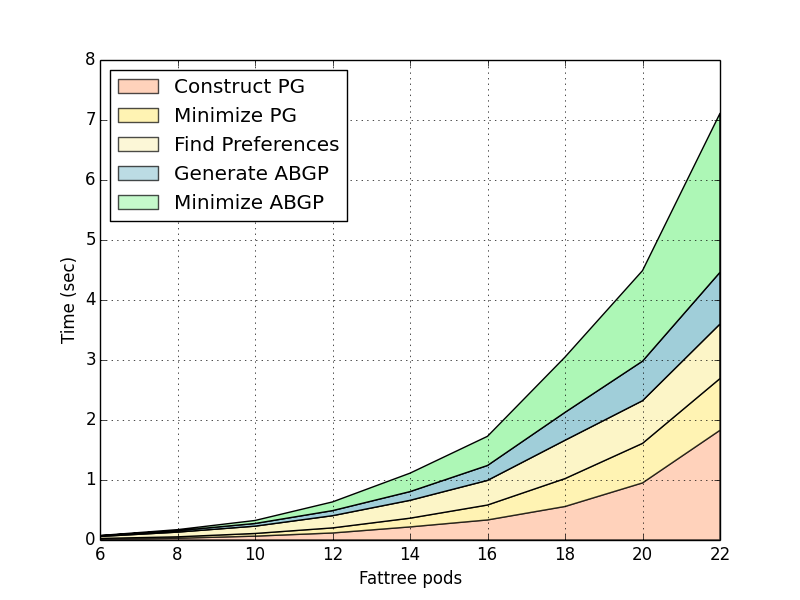
\includegraphics[width=\columnwidth]{figures/compilation-times-dc.png}
\label{fig:compilation-times-dc}
\caption{Data center compilation times.}
\end{figure}

\begin{figure}[t!]
\centering
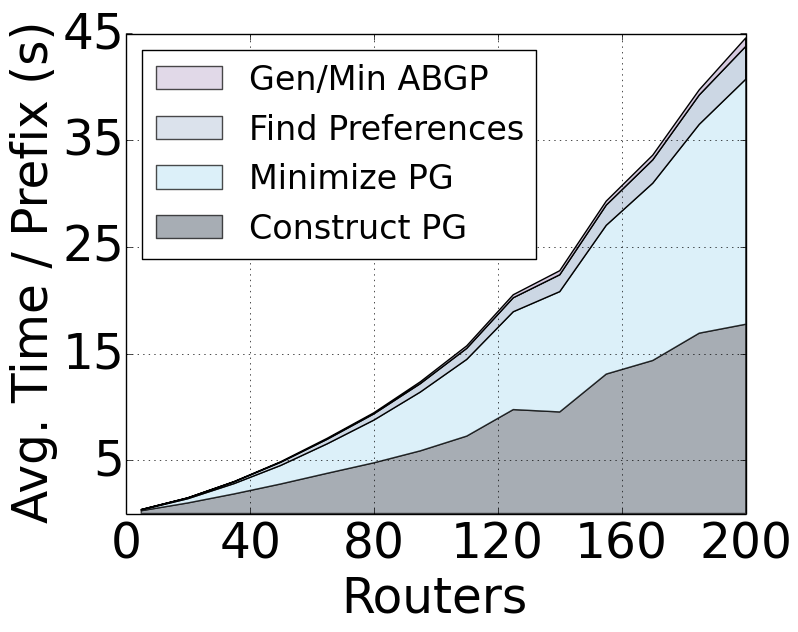
\includegraphics[width=\columnwidth]{figures/compilation-times-backbone.png}
\label{fig:compilation-times-dc}
\caption{Data center compilation times.}
\end{figure}

\begin{figure}[t!]
\centering
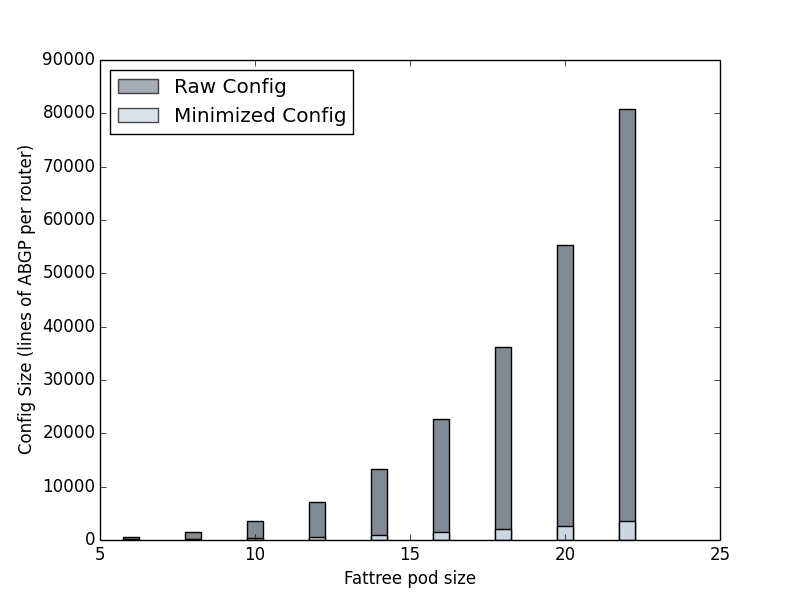
\includegraphics[width=\columnwidth]{figures/config-compression-dc.png}
\label{fig:compilation-compression-dc}
\caption{Data center config minimization.}
\end{figure}

We now study the compilation of time for both policies as a function of network size. Even though the networks we study have a fixed topology and size, we can explore the impact of size because our converted policies are network-wide and the compiler takes topology itself as an input. For the data center network, we build and provide as input fat tree topologies of different sizes, assign a /24 prefix to each ToR switch, and randomly map prefixes to each type of prefix group with a distinct routing policy. We take this approach to smoothly explore different sizes; there is a parameterized way to build fat trees~\cite{fattree}, which does not exist for our concrete data center topologies. For a given size, our reported results match those for the concrete topologies.

For the backbone network, the internal topology does not matter since all routers connect in a full iBGP mesh. We explore different mesh sizes and randomly map neighboring networks to routers.

All experiments are run on an 8 core, 3.6 GHz Intel Xeon processor running Windows 7.
%
For the data center policy, we measure the mean compilation time per-prefix since the \sysname compiler can compile for each prefix independently, and in parallel. Figure~\ref{fig:compilation-times-dc} shows the compilation times for data centers of different sizes, broken down by compilation phase. No individual compilation phase dominates the running time of the compiler, with construction and minimization of the product graph taking the most time. \sysname compiles each data center in under 15 seconds per-prefix on average. Total compilation time for the largest data center with (>1600) routers takes less than 9 minutes total.
\todo{Core compilation times here}

\ryan{Do we want to include this?}
The naive compilation algorithm from \S\ref{sec:compilation} generates extremely large ABGP policies. To offset this, the compiler performs configuration minimization both during and after configuration generation. Such minimization is useful for limiting the computational expense of matching routes on BGP routers, reducing the number of forwarding entries in routers in certain cases, and making configurations more readable for humans. Figure~\ref{fig:compilation-compress-dc} shows the effect of minimization for the data center policy. Minimization significantly reduces the size of the naive configurations.


\subsection{Propane vs. operator configurations}

Finally, we comment briefly on how \sysname-generated configurations differ from those generated by operators today. 
%
In some cases, \sysname configurations are implemented as one would expect. For example, preferences among neighboring ASes are implemented with a compiler-generated community value to tag incoming routes according to preference, which is then observed at other border routers to influence decisions. In other cases, the \sysname configurations are different, relying on a different BGP mechanism to achieve the same result. Some key differences that we observed were: 
%
$i)$ operators used the no-export community to prevent routes from leaking beyond a certain tier of the data center, whereas \sysname selectively imported the route only below a certain tier; 
%\sysname could use a similar implementation mechanism in the future as an optimization.
%
$ii)$ operators prevented unneeded propagation of more-specific route advertisements from a neighboring AS based on their out-of-band knowledge about topology, whereas \sysname propagated these advertisements; and
%
$iii)$ operators used a layer of indirection using community groups and re-writing to implement certain policies in a more maintainable way, where \sysname uses flat communities. We are currently investigating if such differences matter to operators (e.g., if they want to read \sysname configurations) and, if necessary, how to reduce them.


